\chapter{Postprocessing and optimization}

After in previous chapters finding a good model, it is now time to make it great. This chapter is split into two segments: The first considers two detection alternatives and postprocessing methods for accurate recognizing surface transitions, and in the second a few optimizations done to improve the found model are examined.

\section{Postprocessing and detection}

Prediction probabilities are produced by the model in quick succession by interpreting the neural network softmax output as predictive confidences. When the robot passes over a transition region the produced predictions changes, as seen in figure \ref{fig:detect_no}. In order to detect such a change some detection algorithm is required. In this section three such alternatives are compared and evaluated.  


\begin{figure}
	\includegraphics[scale=0.5]{figs_temp/detect_nothing}
	\label{fig:detect_no}
	\caption{Transition region with some outliers}
\end{figure}

\subsection{Thresholding}

The simplest possible detection algorithm is by setting a threshold $\xi$, and classifying below surface as either grass or non-grass depending on whether the prediction is above or below the set threshold. Denoting the resulting prediction as $P$ this detection algorithm is 

\begin{equation}
	P_i=0 \quad\text{if}\quad p_i\leq\xi, \quad
	\text{else} \quad P_i=1
\end{equation}

However, for this method to fail only a single incorrect prediction $p_i$ is required so the algorithm is extremely sensitive to any errors in $p$.

\begin{figure}
	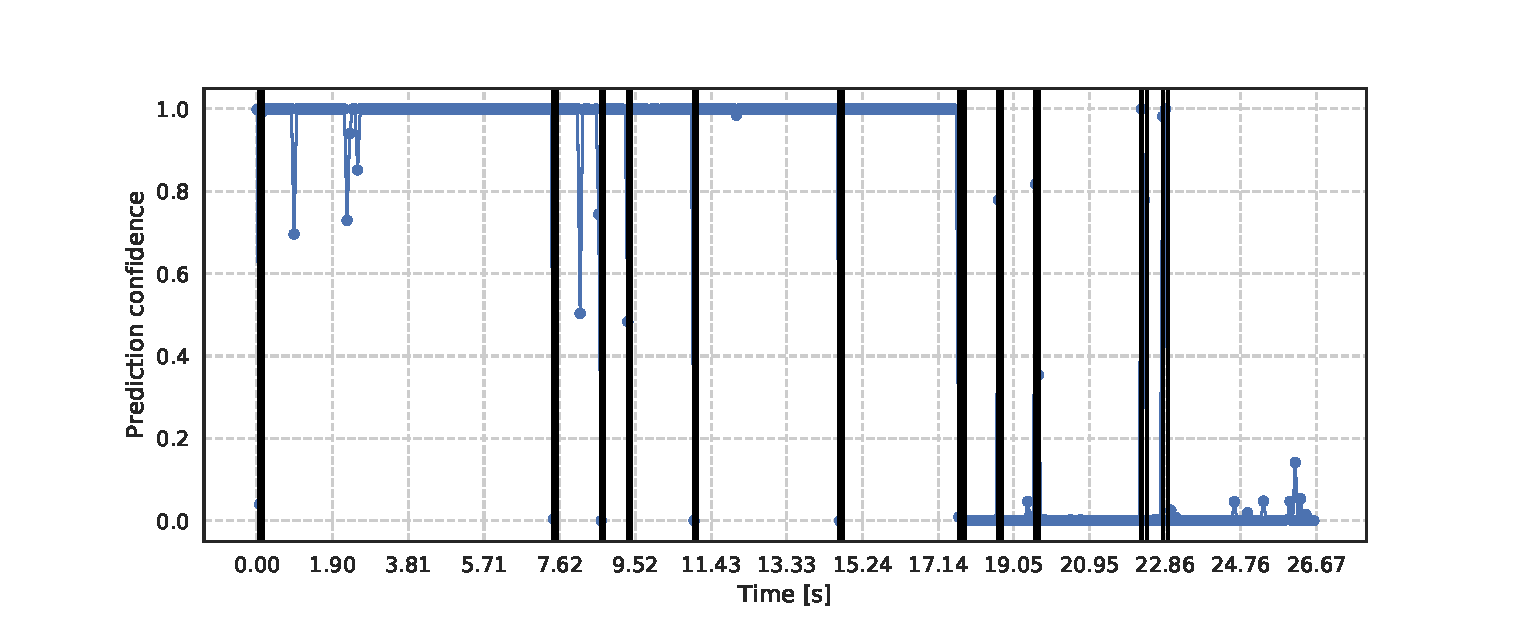
\includegraphics[scale=0.5]{figs_temp/detect_thresh}
	\label{fig:detect_thresh}
	\caption{Detecting transition region using thresholding.}
\end{figure}

\subsection{Median filtering}

The perhaps most effective way of suppressing data littered with outliers is through some form of median filtering. The regular form of a median filter simply takes the median of current and previous datapoints, resulting in an output significantly less sensitive to inconsistencies \citep{pearson_2002}. After median filtering a threshold can be utilized, leading to the following predictions for a filter length $L$

\begin{equation}
	P_i=0 \quad\text{if}\quad\text{median}\{p\}_{i-L+1}^i\leq\xi, 
	\quad \text{else} \quad P_i = 1
\end{equation}

\begin{figure}
	\includegraphics[scale=0.5]{figs_temp/detect_median}
	\label{fig:detect_median}
	\caption{Detection transition using median filtering}
\end{figure}

\subsection{CUSUM}

A traditional and statistically appealing method for effectively detecting abrupt changes in data is CUmulative SUM, hereby refered to as CUSUM. The cumulative sum computed in CUSUM is a log-likelihood $S$ defined through

\begin{equation}
	S_j^k = \sum_{i=j}^k \text{ln}\frac{p_{\theta_1}(y_i)}{p_{\theta_0}(y_i)}
\end{equation}

\begin{figure}
	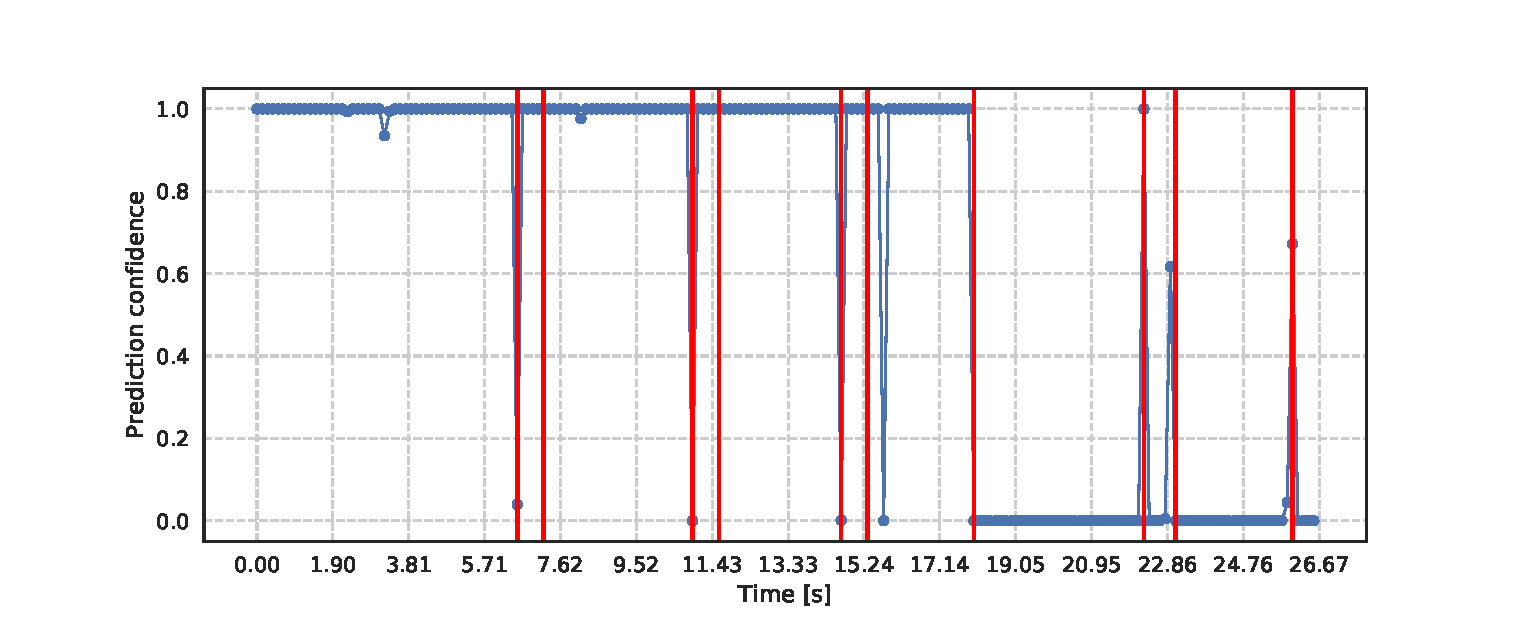
\includegraphics[scale=0.08]{figs_temp/detect_cusum}
	\label{fig:detect_cusum}
	\caption{Detection of transition using CUSUM.}
\end{figure}

[Continue explanation]


\citep{basseville_nikiforov_1993}




\subsection{Method comparison}

After introducing each detection algorithm a comparison is in order. Below is output from a typical transition using [model we made]. Each algorithm has been applied to the data for change detection.


Informal definition as data points inconsistent with our expectations

\section{Removal of outliers}

In any dataset some data corruption is to be expected. A grassy surface may have small patches of soil without grass, the device may have been vibrating unexpectedly for a short period of time or the radar sensor iteslf may have had temporary issues. Erronous data may cause data points inconsistent with the overwhelming bulk of data, which negatively impacts the model accuracy. 

There are multiple ways of identifying and removing outliers. [Only investigate this if we dont go with LSTM!] 

The importance of outliers cannot be overstated. Extreme or influential data points can be significantly detrimental to model accuracy, so effective removal is commonly necessary or at least benifitial \citep{osborne_overbay_2004}, \citep{hodge_austin_2004}. 

\subsection{Mahalanobis distance}

\subsection{DBSCAN}

\section{Hyperparameter optimization}



